\documentclass[aspectratio=169]{beamer}

% Theme selection
\usetheme{Madrid}
\usecolortheme{whale}

% Packages
\usepackage{graphicx}
\usepackage{booktabs}
\usepackage{tikz}
\usetikzlibrary{shapes, positioning, shadows, arrows.meta, fit, backgrounds, calc}
\usepackage{amsmath}
\usepackage{hyperref}
\usepackage{listings}
\usepackage{multirow}
\usepackage{colortbl}

% Custom Colors (from template)
\definecolor{sharifblue}{RGB}{0, 50, 100}
\definecolor{medgreen}{RGB}{40, 140, 40}
\definecolor{alertred}{RGB}{180, 20, 20}
\definecolor{darkred}{RGB}{220, 20, 20}
\setbeamercolor{structure}{fg=sharifblue}
\setbeamercolor{frametitle}{bg=sharifblue, fg=white}

% Title Info
\title[IPL Lab]{CultureCLIP: Empowering CLIP with Cultural Awareness}
\subtitle{Through Synthetic Images and Contextualized Captions}
\author[Shayan Salehi]{Shayan Salehi}
\institute[SUT]{
  Department of Computer Engineering\\
  Sharif University of Technology
}
\date{May 2026}

\begin{document}

%--- Slide 1: Title ---
\begin{frame}
  \titlepage
\end{frame}

%--- Slide 2: Outline ---
\begin{frame}{Outline}
  \tableofcontents
\end{frame}

\section{Introduction \& Problem Statement}

%--- Slide 3: Motivation ---
\begin{frame}{The Challenge of Multimodal Cultural Understanding}
  
  \begin{columns}
    \column{0.55\textwidth}
    \textbf{Vision-Language Models (VLMs) like CLIP:}
    \begin{itemize}
      \item Excel at general cross-modal retrieval and zero-shot classification.
      \item Capture coarse-grained semantics well (e.g., identifying a "dog" or "deity").
      \item \textcolor{alertred}{\textbf{Fail at fine-grained cultural nuances.}}
    \end{itemize}
    
    \vspace{0.3cm}
    \textbf{The "Cultural Gap"}
    \begin{itemize}
      \item Culturally distinct concepts often share overwhelming visual similarities.
      \item VLMs miss subtle, context-dependent visual cues (e.g., accessories, symbolic colors).
      \item Consequence: Mismatches and misclassifications.
    \end{itemize}
    
    \column{0.45\textwidth}
    \begin{block}{The Core Question}
      How can we teach VLMs to capture subtle visual details so they can differentiate between cultural concepts that look similar but mean entirely different things?
    \end{block}
  \end{columns}
  
\end{frame}

%--- Slide 4: Visualizing the Problem ---
\begin{frame}{Visualizing the CLIP Failure Mode}
  \centering
  \vspace{0.2cm}
  \begin{figure}
    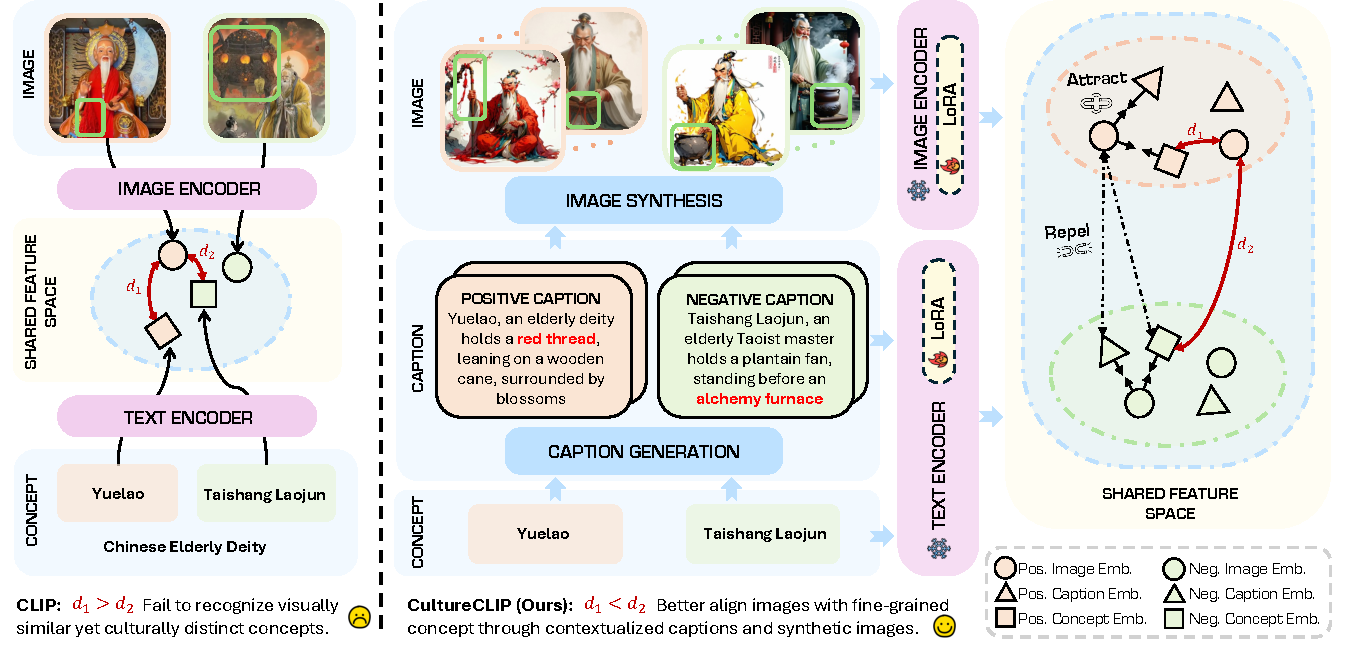
\includegraphics[width=0.7\textwidth]{figures/teaser_cultureclip.pdf}
    \caption{CLIP's embedding space fails to separate visually similar but culturally distinct concepts (e.g., "Sushi" vs. "Gimbap").}
  \end{figure}
\end{frame}

%--- Slide 5: Three Main Challenges ---
\begin{frame}{Three Roadblocks to Cultural Alignment}
  
  \begin{enumerate}
    \setlength{\itemsep}{0.8cm}
    \item \textbf{\textcolor{sharifblue}{Scarcity of High-Quality Cultural Data}}\\
      Manual curation is expensive and small-scale. Web-scraped data is noisy, culturally misleading, and lacks strict alignment.
      
    \item \textbf{\textcolor{sharifblue}{CLIP's Preference for Concise Captions}}\\
      CLIP enforces a 77-token limit. Dense, information-rich cultural context disrupts the alignment learned by the model if naively injected.
      
    \item \textbf{\textcolor{sharifblue}{Absence of Fine-Grained Hard Negatives}}\\
      Standard contrastive learning uses random in-batch negatives. It rarely pairs conceptually similar but visually distinct examples, which are critical for learning cultural boundaries.
  \end{enumerate}
  
\end{frame}

%--- Slide 6: Our Contributions ---
\begin{frame}{Proposed Solution: CulTwin \& CultureCLIP}
  
  \begin{columns}
    \column{0.5\textwidth}
    \textbf{\textcolor{medgreen}{Contribution 1: CulTwin}}
    \begin{itemize}
      \item A highly curated, synthetic cultural dataset.
      \item Features \textbf{Twin Cards}: pairs of concept-caption-image triplets.
      \item Triplets are visually similar but culturally distinct, acting as perfect hard negatives.
    \end{itemize}
    
    \column{0.5\textwidth}
    \textbf{\textcolor{medgreen}{Contribution 2: CultureCLIP}}
    \begin{itemize}
      \item A refined contrastive learning framework.
      \item Jointly aligns concepts, context-rich captions, and synthetic images.
      \item Parameter-efficient fine-tuning (LoRA) to preserve broad VLM generalizations.
    \end{itemize}
  \end{columns}

  \vspace{0.8cm}
  \begin{center}
      \textbf{Goal:} Achieve state-of-the-art fine-grained cultural recognition without losing general domain capabilities.
  \end{center}
  
\end{frame}

\section{CulTwin: Data Curation Pipeline}

%--- Slide 7: CulTwin Pipeline ---
\begin{frame}{CulTwin: A Three-Stage Data Curation Pipeline}
  \centering
  \resizebox{0.95\textwidth}{!}{%
  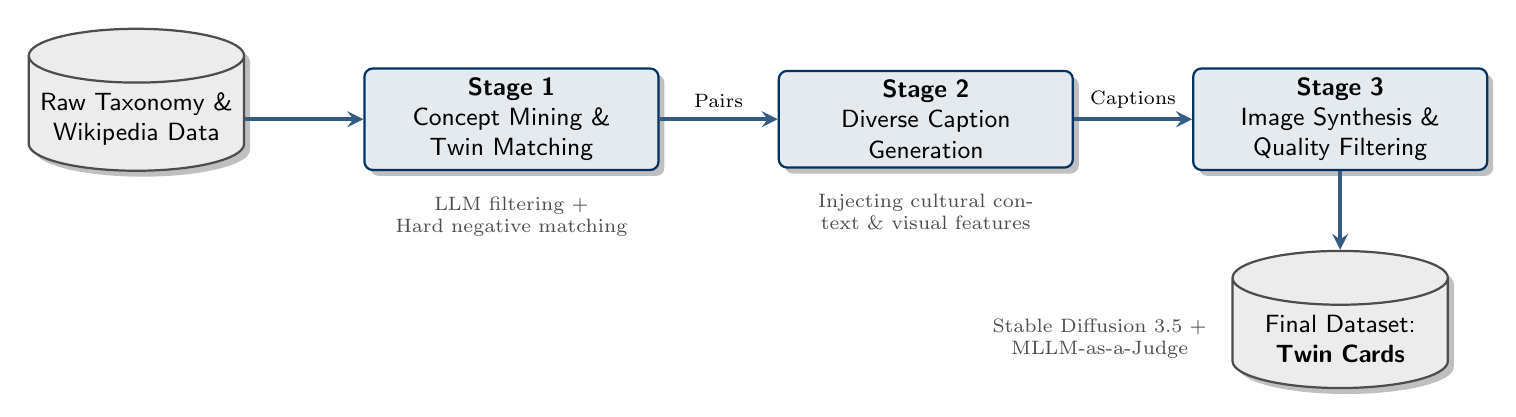
\begin{tikzpicture}[
      node distance=1cm and 1.5cm,
      font=\small\sffamily,
      >=stealth,
      block/.style={rectangle, rounded corners=3pt, draw=sharifblue, thick, fill=sharifblue!10, text width=3.5cm, align=center, minimum height=1.2cm, drop shadow},
      data/.style={cylinder, draw=black!70, thick, fill=gray!15, shape border rotate=90, aspect=0.25, text width=2.5cm, align=center, minimum height=1.2cm, drop shadow},
      arrow/.style={->, line width=1.5pt, draw=sharifblue!80}
  ]
  
  % Nodes
  \node[data] (raw) {Raw Taxonomy \&\\Wikipedia Data};
  \node[block, right=of raw] (stage1) {\textbf{Stage 1}\\Concept Mining \&\\Twin Matching};
  \node[block, right=of stage1] (stage2) {\textbf{Stage 2}\\Diverse Caption\\Generation};
  \node[block, right=of stage2] (stage3) {\textbf{Stage 3}\\Image Synthesis \&\\Quality Filtering};
  \node[data, below=of stage3] (output) {Final Dataset:\\\textbf{Twin Cards}};
  
  % Arrows
  \draw[arrow] (raw) -- (stage1);
  \draw[arrow] (stage1) -- node[above, font=\scriptsize] {Pairs} (stage2);
  \draw[arrow] (stage2) -- node[above, font=\scriptsize] {Captions} (stage3);
  \draw[arrow] (stage3) -- (output);

  % Annotations
  \node[below=0.2cm of stage1, text=black!70, text width=3.5cm, align=center, font=\scriptsize] {LLM filtering +\\Hard negative matching};
  \node[below=0.2cm of stage2, text=black!70, text width=3.5cm, align=center, font=\scriptsize] {Injecting cultural context \& visual features};
  \node[left=-0.2cm of output, text=black!70, text width=3.5cm, align=center, font=\scriptsize] {Stable Diffusion 3.5 +\\MLLM-as-a-Judge};

  \end{tikzpicture}
  }
\end{frame}

%--- Slide 8: Stages 1 & 2 ---
\begin{frame}{Stage 1 \& 2: Concept Mining and Caption Generation}
  
  \textbf{Stage 1: Concept Mining \& Twin Matching}
  \begin{itemize}
    \item \textbf{Taxonomy:} 229 countries across 8 categories (Cuisine, Clothing, Architecture, etc.).
    \item \textbf{LLM Refinement:} We leverage cutting-edge Large Language Models (Qwen2.5-VL) to strictly evaluate cultural relevance.
    \item \textbf{Twin Matching:} The LLM identifies a "cultural twin" for each concept—a hard negative that is visually similar but culturally distinct.
  \end{itemize}

  \vspace{0.4cm}
  
  \textbf{Stage 2: Diverse Caption Generation}
  \begin{itemize}
    \item Generating captions that weave together \textit{both} key visual elements and nuanced cultural background.
    \item \textbf{Diversity Control:} LLM prompts are designed to vary artistic style, lighting, and composition to prevent VLM overfitting on synthetic textures.
  \end{itemize}
  
\end{frame}

%--- Slide 9: Stage 3 ---
\begin{frame}{Stage 3: Image Synthesis \& Quality Filtering}
  
  Images generated via Stable Diffusion 3.5 are rigorously evaluated by an \textbf{MLLM-as-a-Judge} across three dimensions. Scores below a threshold are discarded.
  
  \vspace{0.3cm}
  \begin{table}
    \centering
    \caption{Image Quality Scores (MLLM-as-a-Judge) \& Pass Rates}
    \resizebox{0.9\textwidth}{!}{
      \begin{tabular}{lcccc}
        \toprule
        \textbf{Taxonomy Category} & \textbf{Authenticity $\uparrow$} & \textbf{Consistency $\uparrow$} & \textbf{Fidelity $\uparrow$} & \textbf{Pass \%} \\
        \midrule
        \textbf{Cuisine} & 4.40 & 3.55 & 3.75 & 77.46\% \\
        \textbf{Clothing} & 4.47 & 3.86 & 4.00 & 75.52\% \\
        \textbf{Animals \& Plants} & 4.35 & 3.98 & 4.28 & 75.63\% \\
        \textbf{Art} & 4.39 & 4.03 & 4.09 & 72.67\% \\
        \textbf{Architecture} & 4.22 & 3.90 & 4.00 & 61.32\% \\
        \textbf{Symbol} & 3.80 & 3.83 & 3.98 & \textbf{85.12\%} \\
        \bottomrule
      \end{tabular}
    }
  \end{table}
  
  \vspace{0.2cm}
  \small \textit{Note: Tangible categories (Cuisine/Clothing) yield higher authenticity, while abstract categories (Architecture/Art) face stricter rejection rates.}
\end{frame}

%--- Slide 10: Twin Cards Concept ---
\begin{frame}{The Result: "Twin Cards"}
  
  Each curated instance in CulTwin is a \textbf{Twin Card}: Two opposing triplets of $(C, T, I)$.
  
  \vspace{0.5cm}
  \begin{columns}
    \column{0.41\textwidth}
    \fcolorbox{medgreen}{white}{
      \parbox{\textwidth}{
        \centering
        \textbf{\textcolor{medgreen}{Triplet A (Positive)}}\\
        \vspace{0.2cm}
        \textbf{Concept ($C^+$):} Sushi (Japan)\\
        \vspace{0.1cm}
        \textbf{Caption ($T^+$):} Vinegared rice paired with raw seafood, emphasizing precise cuts and minimalism.\\
        \vspace{0.1cm}
        \textbf{Image ($I^+$):} [Generated Sushi Image]
      }
    }
    
    \column{0.01\textwidth}
    \centering
    \textbf{ VS}
    
    \column{0.41\textwidth}
    \fcolorbox{alertred}{white}{
      \parbox{\textwidth}{
        \centering
        \textbf{\textcolor{alertred}{Triplet B (Hard Negative)}}\\
        \vspace{0.2cm}
        \textbf{Concept ($C^-$):} Gimbap (Korea)\\
        \vspace{0.1cm}
        \textbf{Caption ($T^-$):} Sesame oil-seasoned rice rolled with cooked meats and pickled vegetables.\\
        \vspace{0.1cm}
        \textbf{Image ($I^-$):} [Generated Gimbap Image]
      }
    }
  \end{columns}

  \vspace{0.6cm}
  \textbf{Impact:} The network is forced to learn that the presence of raw fish vs. cooked fillings (visuals) fundamentally alters the cultural concept.
\end{frame}

\section{CultureCLIP: Methodology}

%--- Slide 11: Background ---
\begin{frame}{Preliminaries: Contrastive Alignment Evolution}
  
  \textbf{Standard CLIP Objective:}
  Aligns images $I$ and text $T$ by maximizing cosine similarity for matching pairs while pushing apart random in-batch negatives.
  $$ \mathcal{L}_{\text{CLIP}} = \mathcal{L}_{\text{I2T}} + \mathcal{L}_{\text{T2I}} $$
  
  \textbf{NegCLIP \& TripletCLIP:}
  Introduced explicit hard negative texts $T^-$ (via perturbation) and images $I^-$ to refine decision boundaries.
  $$ \mathcal{L}_{\text{TripletCLIP}} = \mathcal{L}_{\text{NegCLIP}}(I^+, T^+, T^-) + \mathcal{L}_{\text{NegCLIP}}(I^-, T^-, T^+) $$
  
  \begin{alertblock}{The Missing Piece}
  Existing methods focus purely on image-text alignment. They lack an abstract semantic anchor (the \textbf{Concept}) to bind visually nuanced captions and images to their high-level cultural identity.
  \end{alertblock}
  
\end{frame}

%--- Slide 12: Architecture ---
\begin{frame}{CultureCLIP: Architecture \& Alignment}
  \centering
  \resizebox{0.75\textwidth}{!}{%
  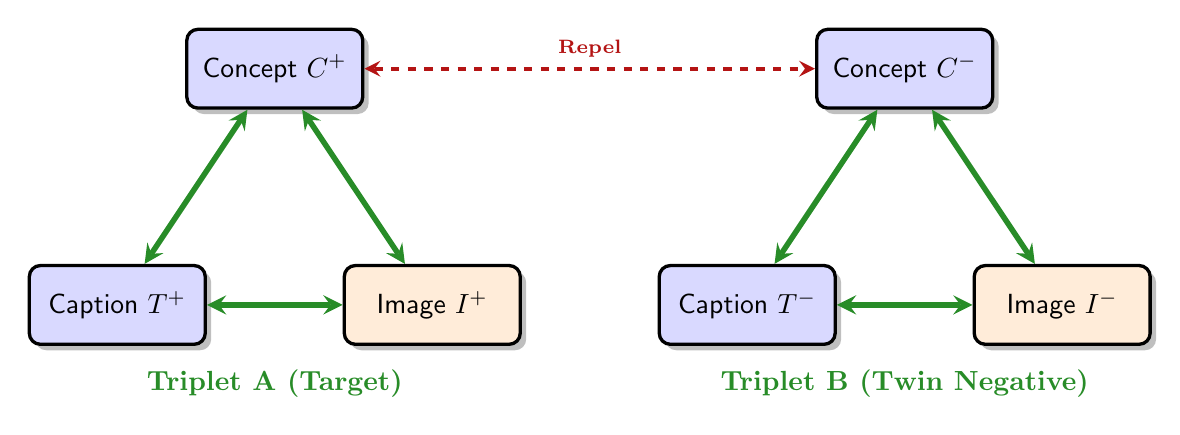
\begin{tikzpicture}[
      font=\sffamily,
      node distance=1.5cm and 2.5cm,
      >=stealth,
      entity/.style={rectangle, rounded corners, draw=black, very thick, text width=2cm, align=center, minimum height=1cm, drop shadow},
      attract/.style={<->, line width=2pt, draw=medgreen},
      repel/.style={<->, dashed, line width=1.5pt, draw=alertred}
  ]
  
  % Triplet A
  \node[entity, fill=blue!15] (ca) at (0,4) {Concept $C^+$};
  \node[entity, fill=blue!15] (ta) at (-2,1) {Caption $T^+$};
  \node[entity, fill=orange!15] (ia) at (2,1) {Image $I^+$};
  
  % Triplet B
  \node[entity, fill=blue!15] (cb) at (8,4) {Concept $C^-$};
  \node[entity, fill=blue!15] (tb) at (6,1) {Caption $T^-$};
  \node[entity, fill=orange!15] (ib) at (10,1) {Image $I^-$};

  % Attraction A
  \draw[attract] (ca) -- (ta);
  \draw[attract] (ca) -- (ia);
  \draw[attract] (ta) -- (ia);

  % Attraction B
  \draw[attract] (cb) -- (tb);
  \draw[attract] (cb) -- (ib);
  \draw[attract] (tb) -- (ib);
  
  % Repulsion (cross)
  \draw[repel] (ca) -- (cb) node[midway, above, font=\scriptsize\bfseries, text=alertred] {Repel};
  % \draw[repel] (ia) -- (tb);
  % \draw[repel] (ib) -- (ta);

  \node[font=\bfseries, text=medgreen] at (0, 0) {Triplet A (Target)};
  \node[font=\bfseries, text=medgreen] at (8, 0) {Triplet B (Twin Negative)};

  \end{tikzpicture}
  }
  
  \vspace{0.4cm}
  Like a magnetic field: Attract components within a cultural triplet; repel elements from the culturally opposing twin.
\end{frame}

%--- Slide 13: Mathematical Formulation ---
\begin{frame}{CultureCLIP Objective Function}
  
  CultureCLIP extends TripletCLIP by treating the abstract \textbf{Concept ($C$)} and detailed \textbf{Caption ($T$)} as dual text anchors sharing the same encoder.
  
  \vspace{0.4cm}
  The overall objective balances concept-level and caption-level losses:
  $$ \mathcal{L}_{\text{CultureCLIP}} = \lambda_c \cdot \mathcal{L}_{\text{concept}} + \lambda_t \cdot \mathcal{L}_{\text{caption}} $$
  
  Where the caption loss enforces text-image alignment against the twin:
  $$ \mathcal{L}_{\text{caption}} = \mathcal{L}_{\text{NegCLIP}}(I^+, T^+, T^-) + \mathcal{L}_{\text{NegCLIP}}(I^-, T^-, T^+) $$
  
  And the concept loss grounds the image to the abstract cultural identity:
  $$ \mathcal{L}_{\text{concept}} = \mathcal{L}_{\text{NegCLIP}}(I^+, C^+, C^-) + \mathcal{L}_{\text{NegCLIP}}(I^-, C^-, C^+) $$
  
\end{frame}

\section{Experiments \& Results}

%--- Slide 14: Experimental Setup ---
\begin{frame}{Experimental Setup}
  
  \textbf{Training Specifications}
  \begin{itemize}
    \item \textbf{Base Model:} CLIP (ViT-B/32 image encoder).
    \item \textbf{Method:} Parameter-Efficient Fine-Tuning using \textbf{LoRA} (Rank 4).
    \item \textbf{Motivation:} Full fine-tuning disrupts general knowledge representations. LoRA adapts efficiently while preserving pre-trained general space.
  \end{itemize}

  \vspace{0.3cm}
  \textbf{Evaluation Benchmarks}
  \begin{itemize}
    \item \textbf{Culture-Specific:} GlobalRG-G, GlobalRG-R, CROPE. \\
          (Adapted into statement-ranking tasks evaluating semantic fine-grain accuracy).
    \item \textbf{Culture-Agnostic:} MS COCO, Flickr30k. \\
          (Testing Recall@5 to ensure standard retrieval abilities aren't forgotten).
  \end{itemize}
  
\end{frame}

%--- Slide 15: Main Results ---
\begin{frame}{Main Results: Overcoming the Cultural Gap}
  
  \begin{center}
    \textbf{Performance on Culture-Specific and Culture-Agnostic Tasks}
    \vspace{0.2cm}
    \resizebox{0.95\textwidth}{!}{
      \begin{tabular}{lccccc}
        \toprule
        \multirow{2}{*}{\textbf{Methods}} & \multicolumn{3}{c}{\textbf{Culture-Specific (Accuracy \%)}} & \multicolumn{2}{c}{\textbf{Culture-Agnostic (R@5)}} \\
        \cmidrule(lr){2-4} \cmidrule(lr){5-6}
        & \textbf{GlobalRG-G} & \textbf{GlobalRG-R} & \textbf{CROPE} & \textbf{MS COCO} & \textbf{Flickr30k} \\
        \midrule
        CLIP (Baseline) & 63.98 & 78.22 & 74.69 & 65.40 & 89.00 \\
        \midrule
        CLIP++ (Naive FT) & 46.05 & 49.98 & 73.62 & 28.80 & 50.80 \\
        NegCLIP++ (Ours) & \underline{66.32} & 78.41 & \textbf{79.25} & \underline{65.50} & \underline{89.20} \\
        \midrule
        \rowcolor{medgreen!10}
        \textbf{CultureCLIP (Ours)} & \textbf{69.47} & \textbf{78.60} & 78.84 & \textbf{66.30} & \textbf{89.30} \\
        \bottomrule
      \end{tabular}
    }
  \end{center}

  \vspace{0.4cm}
  \textbf{Key Takeaways:}
  \begin{itemize}
    \item \textbf{+5.49\%} improvement over base CLIP on GlobalRG-G.
    \item Naive fine-tuning (CLIP++) destroys performance (\textit{Catastrophic Forgetting}).
    \item CultureCLIP improves cultural awareness \textit{and} general retrieval simultaneously.
  \end{itemize}
  
\end{frame}

%--- Slide 16: Ablation - Concept vs Caption ---
\begin{frame}{Ablation: The Role of Concept vs. Caption}

  Which contributes more to fine-grained alignment?
  
  \vspace{0.3cm}
  \begin{center}
    \resizebox{0.85\textwidth}{!}{
      \begin{tabular}{lcccc}
        \toprule
        \textbf{Configuration} & \textbf{$\lambda$ (Cap / Con)} & \textbf{GlobalRG-G} & \textbf{GlobalRG-R} & \textbf{MS COCO} \\
        \midrule
        Caption-only (w/ neg) & 1.0 / -- & 66.27 & 77.53 & 65.50 \\
        Concept-only (w/ neg) & -- / 1.0 & 65.83 & 77.29 & 65.60 \\
        \midrule
        \rowcolor{medgreen!10}
        \textbf{CultureCLIP (Optimal)} & \textbf{0.3 / 0.7} & \textbf{69.47} & \textbf{78.60} & \textbf{66.10} \\
        \bottomrule
      \end{tabular}
    }
  \end{center}

  \vspace{0.5cm}
  \textbf{Insight:} 
  Concepts act as powerful, abstract semantic anchors. Weighting the concept objective higher ($\lambda_c = 0.7$) allows the model to distinguish subtle cultural boundaries better than relying on dense text alone.
  
\end{frame}

%--- Slide 17: Ablation - LoRA & Quality Filtering ---
\begin{frame}{Ablation: LoRA and Data Quality}

  \begin{center}
    \resizebox{0.85\textwidth}{!}{
      \begin{tabular}{lcccc}
        \toprule
        \textbf{Configuration} & \textbf{Quality Filtered} & \textbf{LoRA Rank} & \textbf{GlobalRG-G} & \textbf{CROPE} \\
        \midrule
        Full FT Baseline & $\times$ & -- & 46.95 & 73.62 \\
        Full FT + QF & \checkmark & -- & 43.64 & 74.33 \\
        LoRA Baseline & $\times$ & 4 & \underline{69.47} & 78.84 \\
        \midrule
        \rowcolor{medgreen!10}
        \textbf{CultureCLIP (+QF + LoRA)} & \checkmark & \textbf{4} & \textbf{69.67} & \textbf{79.21} \\
        \bottomrule
      \end{tabular}
    }
  \end{center}

  \vspace{0.4cm}
  \textbf{Insights:}
  \begin{itemize}
    \item \textbf{LoRA is strictly necessary} to prevent catastrophic forgetting. Full parameter updates on domain-specific data destroy pre-trained manifolds.
    \item \textbf{Quality filtering works:} Training on 73.8k high-quality filtered samples outperforms the full 100k unfiltered set.
  \end{itemize}

\end{frame}

\section{Conclusion \& Future Work}

%--- Slide 18: Limitations ---
\begin{frame}{Current Limitations}
  
  \begin{itemize}
    \setlength{\itemsep}{0.6cm}
    \item \textbf{Highly Abstract Reasoning:} CultureCLIP still struggles when visual distinctions are purely stylistic or symbolic rather than physically concrete.
    \item \textbf{Evaluation Bottleneck:} Relying on MLLMs (like Qwen2.5-VL) as judges introduces potential model biases and restricts true interpretability.
    \item \textbf{The Synthetic Domain Gap:} While highly diverse, CulTwin is fully synthetic. A distributional shift exists between generated imagery and real-world, in-the-wild cultural photographs.
  \end{itemize}
  
\end{frame}

%--- Slide 19: Conclusion ---
\begin{frame}{Conclusion \& Takeaways}
  
  \begin{enumerate}
    \setlength{\itemsep}{0.6cm}
    \item \textbf{CulTwin Dataset:} A novel, scalable pipeline for generating synthetic cultural data, leveraging cutting-edge LLMs and Diffusion models to create hard "Twin Card" negatives.
    \item \textbf{CultureCLIP Architecture:} A refined contrastive learning objective that explicitly anchors detailed visual/textual information to high-level cultural concepts.
    \item \textbf{State-of-the-Art Results:} Demonstrated significant improvements on culture-specific benchmarks (+5.49\%) while simultaneously enhancing general zero-shot retrieval capabilities.
  \end{enumerate}

  \vspace{0.8cm}
  \begin{center}
      \large \textbf{Thank You!}
  \end{center}
  
\end{frame}

%--- Slide 20: References ---
\section{References}
\begin{frame}[allowframebreaks]{References}
  \scriptsize
  \bibliographystyle{plain}
  \begin{thebibliography}{99}
  \bibitem{radford2021learning} Radford, A., et al. (2021). Learning Transferable Visual Models From Natural Language Supervision. \emph{ICML}.
  \bibitem{yuksekgonul2022and} Yuksekgonul, M., et al. (2022). When and Why Vision-Language Models Behave like Bags-of-Words, and What to Do About It?. \emph{ICLR}.
  \bibitem{patel2024tripletclip} Patel, et al. (2024). TripletCLIP: Improving Fine-grained Concept Understanding.
  \bibitem{bai2025qwen25vltechnicalreport} Bai, et al. (2025). Qwen2.5-VL Technical Report.
  \bibitem{rombach2022highresolutionimagesynthesislatent} Rombach, R., et al. (2022). High-Resolution Image Synthesis with Latent Diffusion Models. \emph{CVPR}.
  \bibitem{hu2021loralowrankadaptationlarge} Hu, E. J., et al. (2021). LoRA: Low-Rank Adaptation of Large Language Models. \emph{ICLR}.
  \end{thebibliography}
\end{frame}

\end{document}